\chapter{Results}\label{chap:results}
The optimized design of Section~\ref{sec:struct-shared} was synthesized for different network parameters, using Xilinx's Vivado 2015.4 Design Suite,
and the synthesis results are reported in Section~\ref{sec:res-synth}, along with their discussion. The performance of the synthesized networks is very promising,
showing an approximate $251\times$ speed-up over the LSTM Python model, which was running on a high-end desktop computer with an overclocked CPU, and a $14\times$ speed-up
over the most recent hardware implementation~\cite{Chang15} Although the FPGA aims for an Embedded System environment usage, the fairness of the comparison with a Desktop computer
still holds, since a Python/Numpy implementation is slower than a lower-level language implementation (such as in C) and this level of performance would be similar to a C implementation
in a low-power, embedded CPU platform. These results are reported in Section~\ref{sec:res-valid}.

\section{Synthesis}\label{sec:res-synth}
The proposed network was first synthesized aiming a Xilinx XC7Z020 SoC, for sizes $N$ of 4, 8, 16 and 32, varying the resource sharing parameter $K_G$, and the number of inputs set
to $M=2$. For a network size of 32 and $K_G=8$, the LUT usage exceeded the LUT resources available in the FPGA, so only lower values of $K_G$ were
successfully synthesized. This is because of the complexity of the input multiplexer of the Matrix-vector Dot Product Module in~\ref{sec:dotprod_sec}. To synthesize the
design for sizes $N$ of 64, 128 and 256, a Virtex-7 VC707 board was used.

In order to assess the impact of the network size on the performance and resource usage of the proposed design, the Verilog description of the proposed network was first synthesized
aiming a Xilinx XC7Z020 SoC platform, for sizes $N \in \left\{4, 8, 16, 32 \right\}$, and for each of these the resource sharing parameter $K_G$ was also varied (as will be explained further ahead,
the number of inputs is set to $M=2$). Since performance is the key factor for using an FPGA implementation, the synthesis strategy used was the \verb+Flow_PerfOptimized_high+, and the implementation
strategy was \verb+Performance_ExplorePostRoutePhysOpt+ to perform a post-route optimization stage that proved useful in many cases to meet the clock specifications when the first Place\&Route pass
failed to meet them. For a network size of 32 and $K_G=8$, the LUT usage exceeded the LUT resources available in the FPGA, so only lower values of $K_G$ were successfully synthesized (N.D. in the tables).
Networks of sizes $N \in \left\{64, 128\right\}$ were also synthesized for a Virtex-7 VC707 board.

\subsection{Maximum Frequency}\label{sec:res-synth-maxfreq}
Using the synthesis strategy outlined in the previous paragraph, the maximum clock frequency that does not cause timing violations of any sort is plotted in
Figure~\ref{fig:maxfreq}. For $N=4$, since there are only 4 rows to be multiplied, the maximum value of $K_G$ is 4, and hence no synthesis was performed for $K_G = 8$ (N.A. in the tables);
also, since $K_G = 2$ and $N=32$ would use $32(8/2+3) = 224$ DSP slices, that exceeds the 220 slices available in the Zynq 7020, so there is no synthesis data for that value.

First, for all network sizes, it is clear that with increasing $K_G$, the maximum clock speed decreases. This means that there is a critical path in the Matrix-Vector multiplication unit,
whose multiplexer becomes increasingly complex for higher values of $K_G$. On the other hand, when $K_G$ is the same, smaller networks are faster than larger networks. The fastest design
is an $N=4$ and $K_G = 2$ network, with a clock frequency of $158.228$ MHz, and the slowest one is an $N=32$ and $K_G=4$ network, clocked at $101.523$ MHz. The reference design used for
validation in Section~\ref{sec:res-valid} is an $N=8$ and $K_G=2$ network is clocked at $154.321$ MHz, which yields a clock period of $6.48$ ns.

\begin{figure}
    \centering
    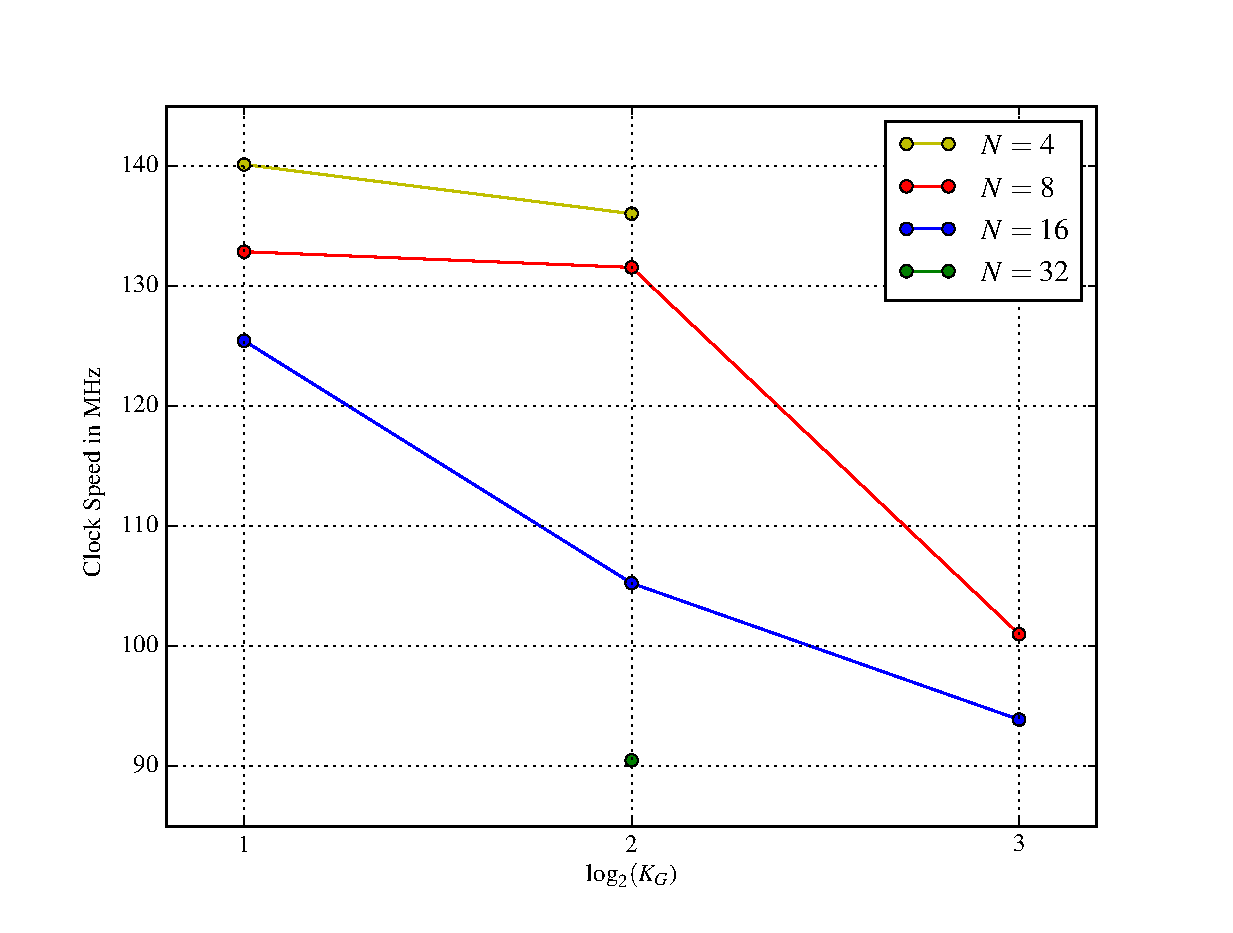
\includegraphics[width=\linewidth]{figures/maxfreq.eps}
    \caption[The maximum achievable clock frequency for several Network Sizes $N$ and resource sharing level $K_G$]{The maximum achievable clock frequency for several Network Sizes $N$ and resource sharing level $K_G$}
    \label{fig:maxfreq}
\end{figure}


\subsection{DSP Slices Usage}\label{sec:res-synth-dsp}
The estimates made in Equation~\ref{eq:numdsp_network-opt} were proven to be accurate, as Figure~\ref{fig:dspused} confirms. The reference network design uses 56 DSP slices, which
corresponds to $25.45\%$ of the total number of DSP slices available.

\begin{figure}
    \centering
    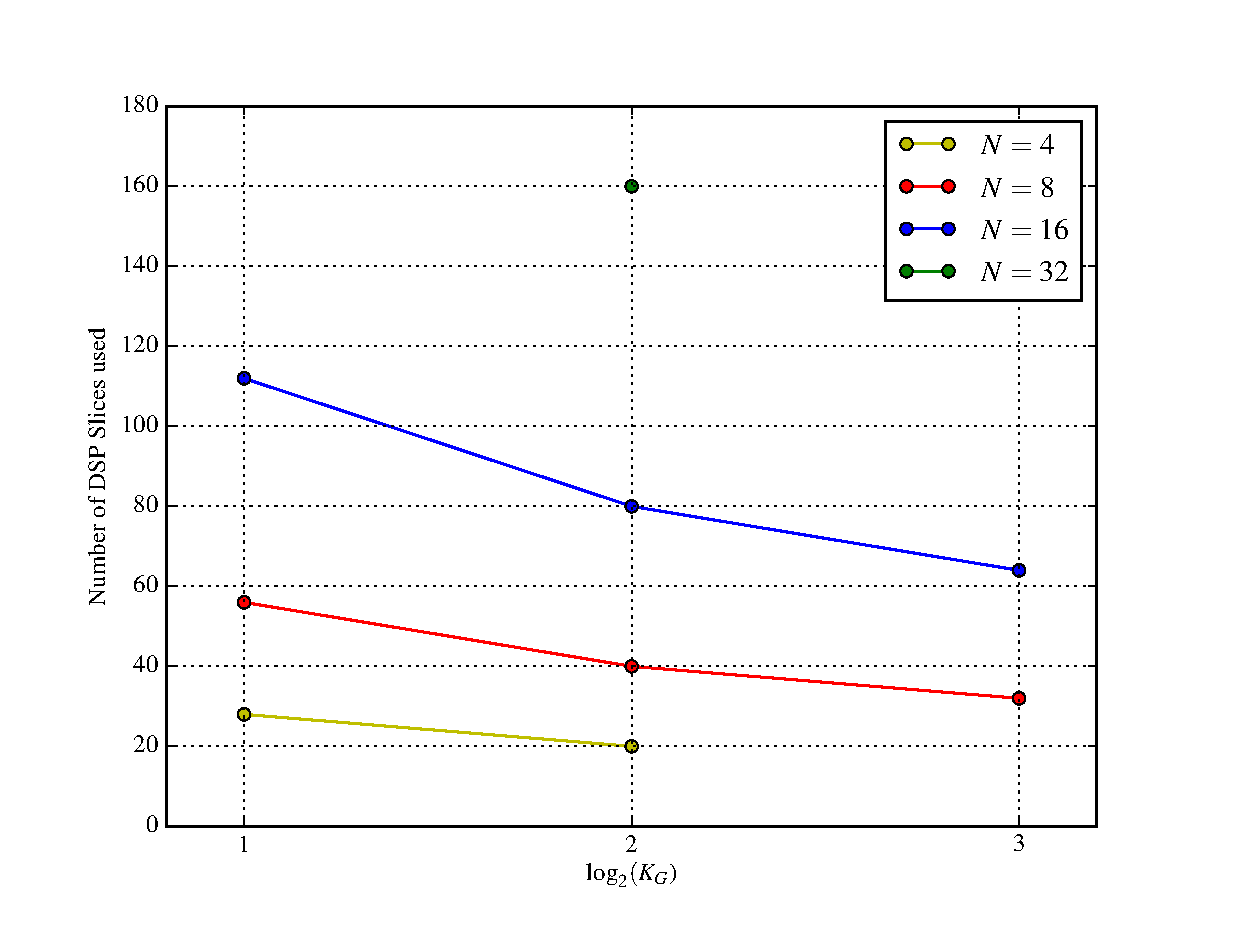
\includegraphics[width=\linewidth]{figures/dspuse.eps}
    \caption[The number of DSP slices used for several Network Sizes $N$ and resource sharing level $K_G$]{The number of DSP slices used for several Network Sizes $N$ and resource sharing level $K_G$}
    \label{fig:dspused}
\end{figure}

\subsection{Power Consumption}\label{sec:res-synth-power}
Another important metric of the performance of a design is its \textbf{power consumption}. All designs yielded a constant baseline value for the \emph{static} power consumption of around 120 mW,
and the power consumption reported in Figure~\ref{fig:power} refers to the \emph{total} power consumptions, i.e. both the baseline static power and the dynamic power consumption.
It is clear that the smaller the network is, the less power is consumed, as one would expect. Furthermore, an increasing level of resource sharing, $K_G$, yields a substantially lower
power consumption figure: this is because less DSP slices are used when $K_G$ is increased. Of course, even though the power consumption is lower in that case, that comes at the
expense of a lower clock frequency and a higher computation overhead per forward propagation.

\begin{figure}
    \centering
    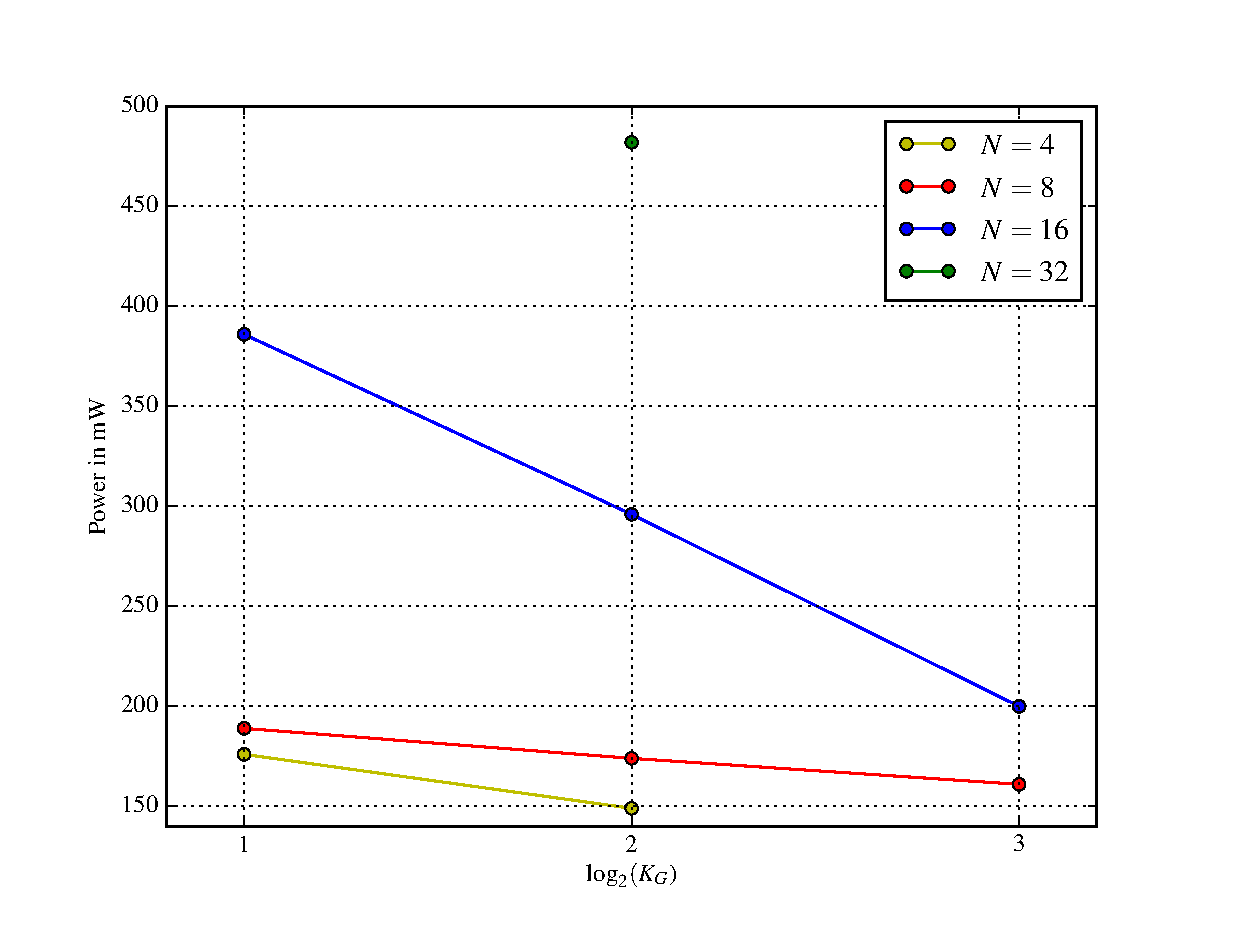
\includegraphics[width=\linewidth]{figures/power.eps}
    \caption[Power consumption estimates for several Network Sizes $N$ and resource sharing level $K_G$]{Power Consumption estimates for several Network Sizes $N$ and resource sharing level $K_G$}
    \label{fig:power}
\end{figure}

\subsection{Other Resources Usage}\label{sec:res-synth-otheres}
The LUT, LUTRAM and Flip-Flop usages are discussed here. In Table~\ref{tab:lut}, the usage of LUTs is reported, where we can see
that although there is not a clear trend on how the LUT usage varies with increasing $K_G$, it is clear, and expectable, that
the LUT usage increases with the size of the network by an approximate factor of 2, from $N=2$ to $N=16$. As for $N=32$, the
usage does not follow this apparent trend, and rises sharply to 91\%. For $K_G = 8$ the usage surpasses the maximum amount
of LUTs available in the XC7Z020.

\begin{table}

    \centering
  \begin{tabular}{ | l | c | c | c |}
    \hline
    & $K_G=2$  & $K_G=4$ & $K_G=8$ \\
    \hline
    $N=4$ & 6.87\% & 6.04\% & N.A. \\
    \hline
    $N=8$ & 14.64\% & 13.03\% & 14.11\% \\
    \hline
    $N=16$ & 28.97\% & 27.72\% & 29.85\% \\
    \hline
    $N=32$ & N.A. & 91.09\% & N.D. \\
\hline
  \end{tabular}
  \caption{LUT usage for different $N$ and $K_G$ in the XC7Z020}
  \label{tab:lut}
\end{table}

As for LUTs, the FF usage also scales accordingly to a $2\times$ factor. In terms of LUTRAM, used to store the network weights,
the amount used increases by 2 with increasing values of $N$, as before, and \textbf{does not} depend on $K_G$. This is because
the amount of weights only depends on the network sizes $M$ and $N$, and not on $K_G$. Furthermore, unlike LUTs, it scales well
with increasing network sizes, and does not pose a limitation on the network size. The usage results for the XC7Z020 are reported in Table~\ref{tab:ff},
and in Table~\ref{tab:ff-virtx7} the usages for the VC707.

\begin{table}
    \centering
  \begin{tabular}{ | l | c | c |}
    \hline
         & LUTRAM  & FF  \\
    \hline
    $N=4$ & 0.18\%  & 3.39\% \\
    \hline
    $N=8$ & 4.41\%  & 6.7\% \\
    \hline
    $N=16$ & 8.83\%  & 13.36\% \\
    \hline
    $N=32$ & 17.66\% &  26.45\% \\
\hline
  \end{tabular}
  \caption{Flip-flop and LUTRAM usage for the XC7Z020}
	\label{tab:ff}
\end{table}


\begin{table}

    \centering
  \begin{tabular}{ | l | c | c | c |}
    \hline
         & LUTRAM  & FF & LUT \\
    \hline
    $N=64$ & 24.22\%  & 9.14\% & 24.22\% \\
    \hline
    $N=128$ & 14.09\%  & 18.3\% & 41.82\%\\
    \hline
  \end{tabular}
  \caption{Flip-flop, LUTRAM and LUT usage for the VC707}
  \label{tab:ff-virtx7}
\end{table}

\section{Validation and Comparison}\label{sec:res-valid}
Over the course of this Section, the functionality of the network is verified against the Python reference module of~\ref{sec:res-pyth} that was developed as a
reference, both for the forward propagation of the network, as well as for the training algorithm. The methodology of this procedure is outlined in Section~\ref{sec:res-meth}.
On Section~\ref{sec:res-valid-fpps}, the performance results of Section~\ref{sec:res-synth-maxfreq} is translated into how many classifications per second this design
achieves, and how that figure compares with the capabilities of the Python module and the current existing hardware implementation~\cite{Chang15}.

\subsection{Reference Python Module}\label{sec:res-pyth}
Before performing the Verilog description of the network, the ideas outlined in Section~\ref{chap:theorBack} were tested first by building a software version of an LSTM Network.
Since we want to quickly test the ideas without much effort, Python and Numpy were used rather than MATLAB, since Python/Numpy has higher performance at the same level of
code complexity. The code for this Python class is listed in Appendix~\ref{ap1:lstm-pyth}. It supports both the forward propagation of an already trained network, but also provides
functions to train a model using the SPSA method outlined in Section~\ref{sec:training_lstm} and also Backpropagation Through-Time as presented in~\cite{Greff15}. As the reader can attest
by running the code himself, the SPSA proves to be a valid approach for training these networks, achieving convergence for the Machine Learning task that will be presented in the next paragraph,
although it converges slower than Backpropagation Through Time.

The learning problem presented to both the software and hardware network is the sum of two binary numbers of 8 bits. The bits of each number at position $i$ are input to the network as a vector,
and the network outputs its prediction of the correct value of the $i$-th bit of the \emph{result} number. After the whole number number is processed, the memory cells of the LSTM network are reset
and a new addition task can be presented to the network. Even though this seems a rather simple problem, it accounts for all the essential issues at which this network excels: first, this is
a \emph{classification} problem in which the Machine Learning algorithm needs to output a prediction based on the input feature vector, and that prediction has to take into account the \emph{history}
of predictions so far, because the current bit is the sum of not only the bits of the two operands, but also the \emph{carry} generated at the last few positions -- this is where the memory cells of
this special Neural Network come into effect.

\subsection{Methodology}\label{sec:res-meth}
The Python testbench that both trains and verifies the predictions of the software network of Appendix~\ref{ap1:lstm-pyth} is listed in Appendix~\ref{ap1:testbench-pyth}. The scripts train the
network for a maximum of 100 epochs, and in each epoch, the network is presented with 5000 8 bit additions for training, and then 100 8 bit additions for testing, where the prediction error is
calculated, and the training convergence is verified (when there is zero error for two consecutive times). After achieving convergence, the script stores the trained network weights in
\href{https://docs.python.org/3/library/pickle.html}{Pickle} format. These weights are, then, converted to $Q6.11$ fixed-point format and directly loaded into the Verilog model by the Verilog
testbench. The Verilog testbench then applies in order the bits of randomly generated numbers, captures the output bit and checks
whether it is correct or not, and counts the number of incorrect bits.

This network has, then, two inputs ($M=2$) and eight neurons ($N=8$). Furthermore, the output of the eight LSTM neurons is reduced to a single output by means of a simple neuron, as the one
described in Figure~\ref{fig:modelNeuron_a}. This introduces a further 5 clock cycle overhead that is not accounted in Section~\ref{sec:res-valid-fpps}, since it is not actually part of the
LSTM Network. Although it was placed in series in the datapath, after the LSTM network, it can be run in parallel with the LSTM network, introducing no overhead whatsoever.

A Python script was written (see Appendix~\ref{ap1:runtb-lstm}) to automatically compile the Verilog code, generate the input and output data, and call Questasim to run the simulation of the
HDL code. Figure~\ref{fig:res-meth-wave} shows the waveform viewer window of a run of the Verilog testbench, and in Appendix~\ref{ap1:transcript-cmd} shows the transcript of a successful
run of this testbench, proving that the learning ability of the Hardware network still retains the predicting capability of the software network.

\begin{sidewaysfigure}
    \centering
    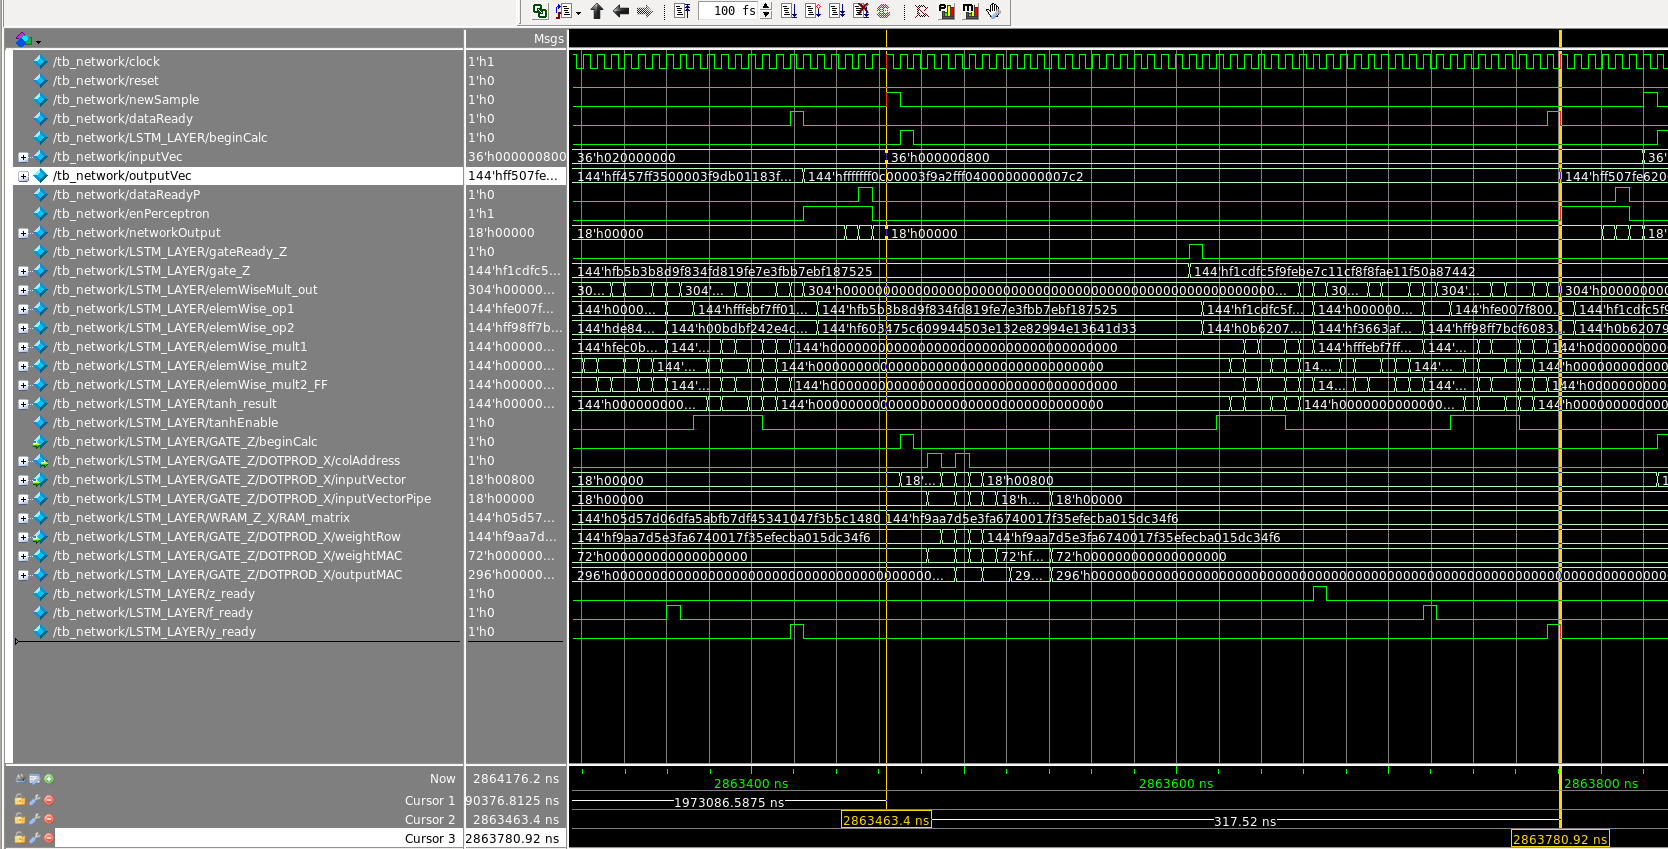
\includegraphics[width=\linewidth]{figures/wave.png}
    \caption[Screenshot of the simulation run of a complete forward propagation for $N=8$ and $K_G=2$]{Screenshot of the simulation run of a complete forward propagation for $N=8$ and $K_G=2$. The period between the two time cursors is the same as the one reported in Table~\ref{tab:process-time}}
    \label{fig:res-meth-wave}
\end{sidewaysfigure}

\subsection{Performance}\label{sec:res-valid-fpps}
To evaluate the performance, a metric was defined based on how many predictions it can produce per second (i.e. produce a new result bit in the output sequence),
in \textbf{millions}. The metric on~\cite{Chang15} is not very informative, since
although a system can perform many calculations per second, if those operations are redundant, that metric has no relevant information
regarding \textbf{how fast} the system can \textbf{perform the actual task it was meant to do}, which in this case is a complete Forward
Propagation through the network. The prediction time is the time elapsed since a new input vector is applied \emph{to} the moment the LSTM
Network produces an output vector. Hence, we multiply the number of clock cycles yielded by Equation~\ref{eq:numcc_network-opt} by the equivalent clock period
from the synthesis clock report of Figure~\ref{fig:maxfreq}.
This result is epitomized in Table~\ref{tab:process-time}, where the calculation time of the Python module's Forward Propagation function is
also included. This time was measured using the \textbf{timeit}\footnote{https://docs.python.org/3.5/library/timeit.html}  module, that allows
the evaluation of the execution time of small pieces of code as well as complete functions with arguments. The Python code was run on a Linux System,
powered by an i7-3770k Intel Processor, running at 4.2GHz.

\begin{table}
    \centering
    \begin{tabular}{ | l | c | c | c | c | c | }
    \hline
    & $K_G=8$  & $K_G=4$ & $K_G=2$ & Python & Speed-up \\
    \hline
    $N=4$ & N.A.  & 309.68 ns  & 259.12 ns & 65 $\mu$s & $\times251$ \\
    \hline
    $N=8$ & 793.46 ns  & 421.12 ns  &  317.52 ns & 72 $\mu$s & $\times228$ \\
    \hline
    $N=16$ & 1.497 $\mu$s  & 738.19 ns  & 461.336 ns & 96 $\mu$s & $\times208$ \\
    \hline
    $N=32$ & N.D.          & 1.586 $\mu$s & N.A.       & 185 $\mu$s  &  $\times117$ \\
		\hline
  \end{tabular}
  \caption{Total processing time for a single forward propagation on the XC7Z020}
  \label{tab:process-time}
\end{table}
The performance increase is significant, even for the slowest of the designs (the $N=32$ network). The hardware network is, at best, $\times251$ faster than the software counterpart,
and at worst $\times117$ faster. Also, it is noticeable that increasing the level of resource sharing increases the computation time, since the level of parallelism is lower.

Since the previous values are the time needed for a \emph{single} forward propagation, to know how many forward propagations we can perform \emph{per second},
we only need to invert the previous values. These values are presented in Figure~\ref{fig:Mclass-psec}. While the $N=8$ and $K_G=2$ network is able to
perform around 3.15 million predictions per second, the Python model can only output around 14 thousand predictions, which is a very significant result that
proves the relevance of this implementation.

\begin{figure}
    \centering
    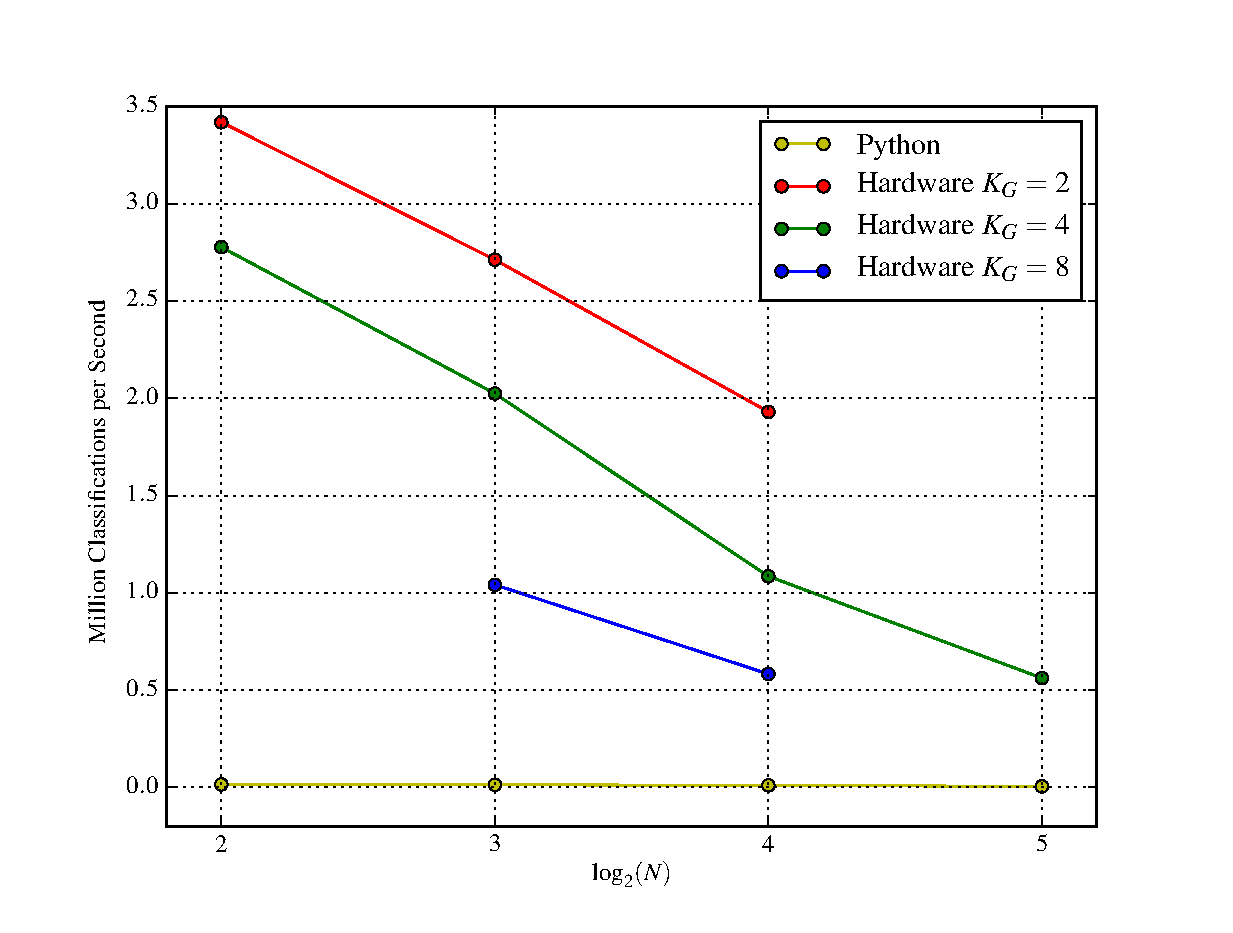
\includegraphics[width=\linewidth]{figures/Mclass-psec.eps}
    \caption[Millions of classifications per second of each design according to the network size $N$]{Millions of classifications per second of each design according to the network size $N$. The comparison is between the software Python model and 3 networks of different levels of resource sharing $K_G$.}
    \label{fig:Mclass-psec}
\end{figure}

As for the larger-sized networks synthesized in the VC707, the results are also very promising. For network sizes of $N=64$ and $N=128$, a complete
forward propagation takes 1.14 $\mu$s and 2.052 $\mu$s respectively, and for both the maximum clock frequency achievable was 140.845 MHz. Since the
design~\cite{Chang15}, for $N=128$, takes an estimated 29.13 $\mu$s, this design yields an improvement of $14\times$ over it.
